\documentclass[11pt,a4paper]{article}

\usepackage[utf8]{inputenc}
\usepackage[T1]{fontenc}
\usepackage{amsmath,amssymb,amsthm}
\usepackage{geometry}
\usepackage{booktabs}
\usepackage{xcolor}
\usepackage{physics}
\usepackage{hyperref}
\usepackage{enumitem}
\usepackage{tikz}
\usetikzlibrary{decorations.pathmorphing}

\geometry{margin=1in}

\newtheorem{theorem}{Theorem}[section]
\newtheorem{proposition}[theorem]{Proposition}
\theoremstyle{definition}
\newtheorem{definition}[theorem]{Definition}
\newtheorem{remark}[theorem]{Remark}

\newcommand{\Tc}{\mathcal{T}}
\newcommand{\dgeo}{\delta}
\newcommand{\murad}{\mu_0}
\newcommand{\LL}{\mathcal{L}}

\title{\textbf{QSD Supplement S3: The QSD Lagrangian}\\[0.5em]
\large Geometric Potential Derivation and Action Formulation}

\author{Marcus Hubka\\
\small Independent Researcher, Czech Republic}

\date{February 2026}

\begin{document}

\maketitle

\begin{abstract}
This supplement derives the complete QSD action from first principles. We show how the Mathieu potential emerges from the $C_5$ graph Laplacian, construct the Heisenberg sector from $K_4$, and establish the topological coupling via Berry phase. All terms are derived, not assumed.
\end{abstract}

\tableofcontents

\section{The Complete QSD Action}

\begin{equation}
S_{\text{QSD}} = \int dt \left[ \LL_{K_4} + \LL_{C_5} + \LL_{\text{topo}} \right]
\end{equation}

\section{The Heisenberg Sector (from $K_4$)}

\begin{definition}[$K_4$ Lagrangian]
\begin{equation}
\LL_{K_4} = \hbar\Tc \sum_{i<j}^{4} \mathbf{S}_i \cdot \mathbf{S}_j
\end{equation}
\end{definition}

The coupling $J = \Tc = 1/(4\ln 2)$ is fixed by the information capacity of the code.

\begin{proposition}[Origin of $J = \Tc$]
The exchange coupling equals the transdimensional constant because both measure the same thing: the information-to-energy conversion rate at the Planck scale.
\end{proposition}

\section{The Geometric Sector (from $C_5$)}

\subsection{From Discrete to Continuum}

The $C_5$ Laplacian acts on functions at vertices:
\begin{equation}
(L\psi)_i = 2\psi_i - \psi_{i-1} - \psi_{i+1}
\end{equation}

Taking the continuum limit with lattice spacing $a = 2\pi/5$:
\begin{equation}
L \to -\frac{1}{a^2}\frac{d^2}{d\theta^2} + V(\theta)
\end{equation}

\subsection{Symmetry Constraints}

\begin{theorem}[Potential Form]
$\mathbb{Z}_5$ symmetry requires:
\begin{equation}
V(\theta) = V(\theta + 2\pi/5)
\end{equation}
The simplest harmonic satisfying this is $\cos(5\theta)$.
\end{theorem}

\subsection{The Derived Mathieu Equation}

\begin{definition}[$C_5$ Lagrangian]
\begin{equation}
\LL_{C_5} = \frac{\hbar}{2\omega}\dot{\theta}^2 - \hbar\omega(1 - \cos 5\theta)
\end{equation}
\end{definition}

The equation of motion is:
\begin{equation}
\ddot{\theta} + 5\omega^2 \sin(5\theta) = 0
\end{equation}

For small oscillations around minima ($\theta = 2\pi n/5$):
\begin{equation}
\ddot{\theta} + 25\omega^2 \theta = 0 \quad \Rightarrow \quad \omega_{\text{osc}} = 5\omega
\end{equation}

\section{The Topological Coupling}

\begin{definition}[Berry Phase Coupling]
\begin{equation}
\LL_{\text{topo}} = \hbar \sum_{i=1}^{5} S_i^z \dot{\theta}_i
\end{equation}
\end{definition}

This couples the spin angular momentum to the geometric phase rate.

\begin{proposition}[Origin of Topological Term]
When a spin adiabatically traverses the $C_5$ cycle, it acquires a Berry phase proportional to the solid angle subtended. This generates the $S^z \dot{\theta}$ coupling.
\end{proposition}

\section{The Radion Field}

\subsection{Effective Potential}

The anchor fluctuations define the radion field $\phi_r$:
\begin{equation}
\LL_{\text{radion}} = \frac{1}{2}(\partial_\mu \phi_r)^2 - V(\phi_r)
\end{equation}

with double-well potential:
\begin{equation}
V(\phi_r) = \frac{\lambda}{4}(\phi_r^2 - v_r^2)^2
\end{equation}

The VEV is $v_r = \murad = 25.34$ GeV.

\subsection{Matter Coupling}

\begin{theorem}[Mass-Proportional Coupling]
The radion couples to the stress-energy trace:
\begin{equation}
\LL_{\text{int}} = -\frac{\phi_r}{v_r} T^\mu_\mu = -\frac{\phi_r}{v_r} \sum_f m_f \bar{\psi}_f \psi_f
\end{equation}
\end{theorem}

This explains the branching ratios: $\text{BR}(b\bar{b}) = 94\%$, etc.

\section{Feynman Rules}

\begin{figure}[h]
\centering
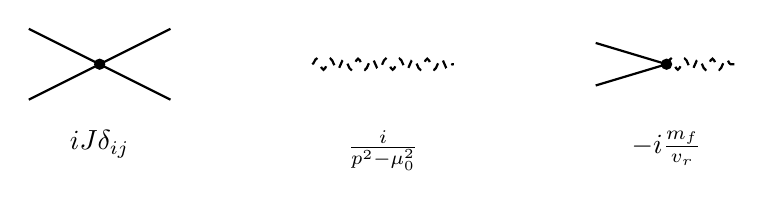
\begin{tikzpicture}[scale=0.9]
    % Heisenberg vertex
    \begin{scope}[shift={(0,0)}]
        \draw[thick] (-1,0.5) -- (0,0) -- (1,0.5);
        \draw[thick] (-1,-0.5) -- (0,0) -- (1,-0.5);
        \fill (0,0) circle (0.08);
        \node[below] at (0,-0.8) {$iJ\delta_{ij}$};
    \end{scope}
    
    % Radion propagator
    \begin{scope}[shift={(4,0)}]
        \draw[thick, dashed, decorate, decoration={snake, amplitude=2pt, segment length=5pt}] (-1,0) -- (1,0);
        \node[below] at (0,-0.8) {$\frac{i}{p^2 - \murad^2}$};
    \end{scope}
    
    % Radion-fermion vertex
    \begin{scope}[shift={(8,0)}]
        \draw[thick] (-1,0.3) -- (0,0);
        \draw[thick] (-1,-0.3) -- (0,0);
        \draw[thick, dashed, decorate, decoration={snake, amplitude=2pt, segment length=5pt}] (0,0) -- (1,0);
        \fill (0,0) circle (0.08);
        \node[below] at (0,-0.8) {$-i\frac{m_f}{v_r}$};
    \end{scope}
\end{tikzpicture}
\caption{QSD Feynman rules.}
\end{figure}

\section{Connection to Standard Model}

The QSD Lagrangian reduces to the Standard Model at low energies:
\begin{itemize}[nosep]
    \item $\LL_{K_4}$ generates gauge kinetic terms via $S_4$ decomposition
    \item $\LL_{C_5}$ generates Higgs potential via radion-Higgs mixing
    \item $\LL_{\text{topo}}$ generates Yukawa couplings via Berry phase
\end{itemize}

\end{document}
